\chapter{Wymagania i diagramy}

\section{wymagania funkcjonalne}
\begin{table}[!h]
	\centering
	\renewcommand{\arraystretch}{1.3}
	\setlength{\tabcolsep}{6pt}
	\begin{tabular}{|c|p{5cm}|p{8cm}|}
		\hline
		\textbf{Nr} & \textbf{Wymaganie funkcjonalne} & \textbf{Opis} \\ \hline
		
		1. & Rejestracja użytkownika & System umożliwia utworzenie konta użytkownika z danymi logowania. \\ \hline
		2. & Logowanie do systemu & System weryfikuje dane użytkownika i umożliwia dostęp do panelu aplikacji. \\ \hline
		3. & Sprawdzenie dostępnych środków & Użytkownik może sprawdzić ile posiada balansu na koncie. \\ \hline
		4. & Wpłata pieniędzy na konto & Użytkownik może zasilić konto. \\ \hline
		5. & Przegląd historii wydatków & Aplikacja wyświetla listę wszystkich wydatków. \\ \hline
		6. & Tworzenie przelewu & System pozwala stworzyć przelew użytkownikowi. \\ \hline
		7. & Podsumowanie finansów konta & Użytkownik może sprawdzić dane o swoich wydatkach dla danego konta. \\ \hline
		
	\end{tabular}
	\caption{Wymagania funkcjonalne systemu do zarządzania budżetem domowym}
	\label{tab:wymagania_funkcjonalne}
\end{table}

\section{wymagania niefunkcjonalne}
\begin{table}[H]
	\centering
	\renewcommand{\arraystretch}{1.3}
	\setlength{\tabcolsep}{6pt}
	\begin{tabular}{|c|p{5cm}|p{8cm}|}
		\hline
		\textbf{Nr} & \textbf{Wymaganie niefunkcjonalne} & \textbf{Opis} \\ \hline
		
		1. & Dostępność & aplikacja ma być dostępna przez 95\% czasu działania serwera \\ \hline
		2. & Wydajność & System reaguje na żądanie w czasie krótszym niż 30 sekund \\ \hline
		3. & Bezpieczeństwo & Hasła muszą być przechowywane w formie zaszyfrowanej. \\ \hline
		4. & Wdrożenie & aplikacja będzie korzystać z Java 21, Spring Boot, React, MongoDB 8.0 \\ \hline
		
	\end{tabular}
	\caption{Wymagania niefunkcjonalne systemu do zarządzania budżetem domowym}
	\label{tab:wymagania_niefunkcjonalne}
\end{table}
\section{Diagramy przypadków użycia}
\textbf{<---Placeholder--->}
\begin{figure}[H]
	\centering
	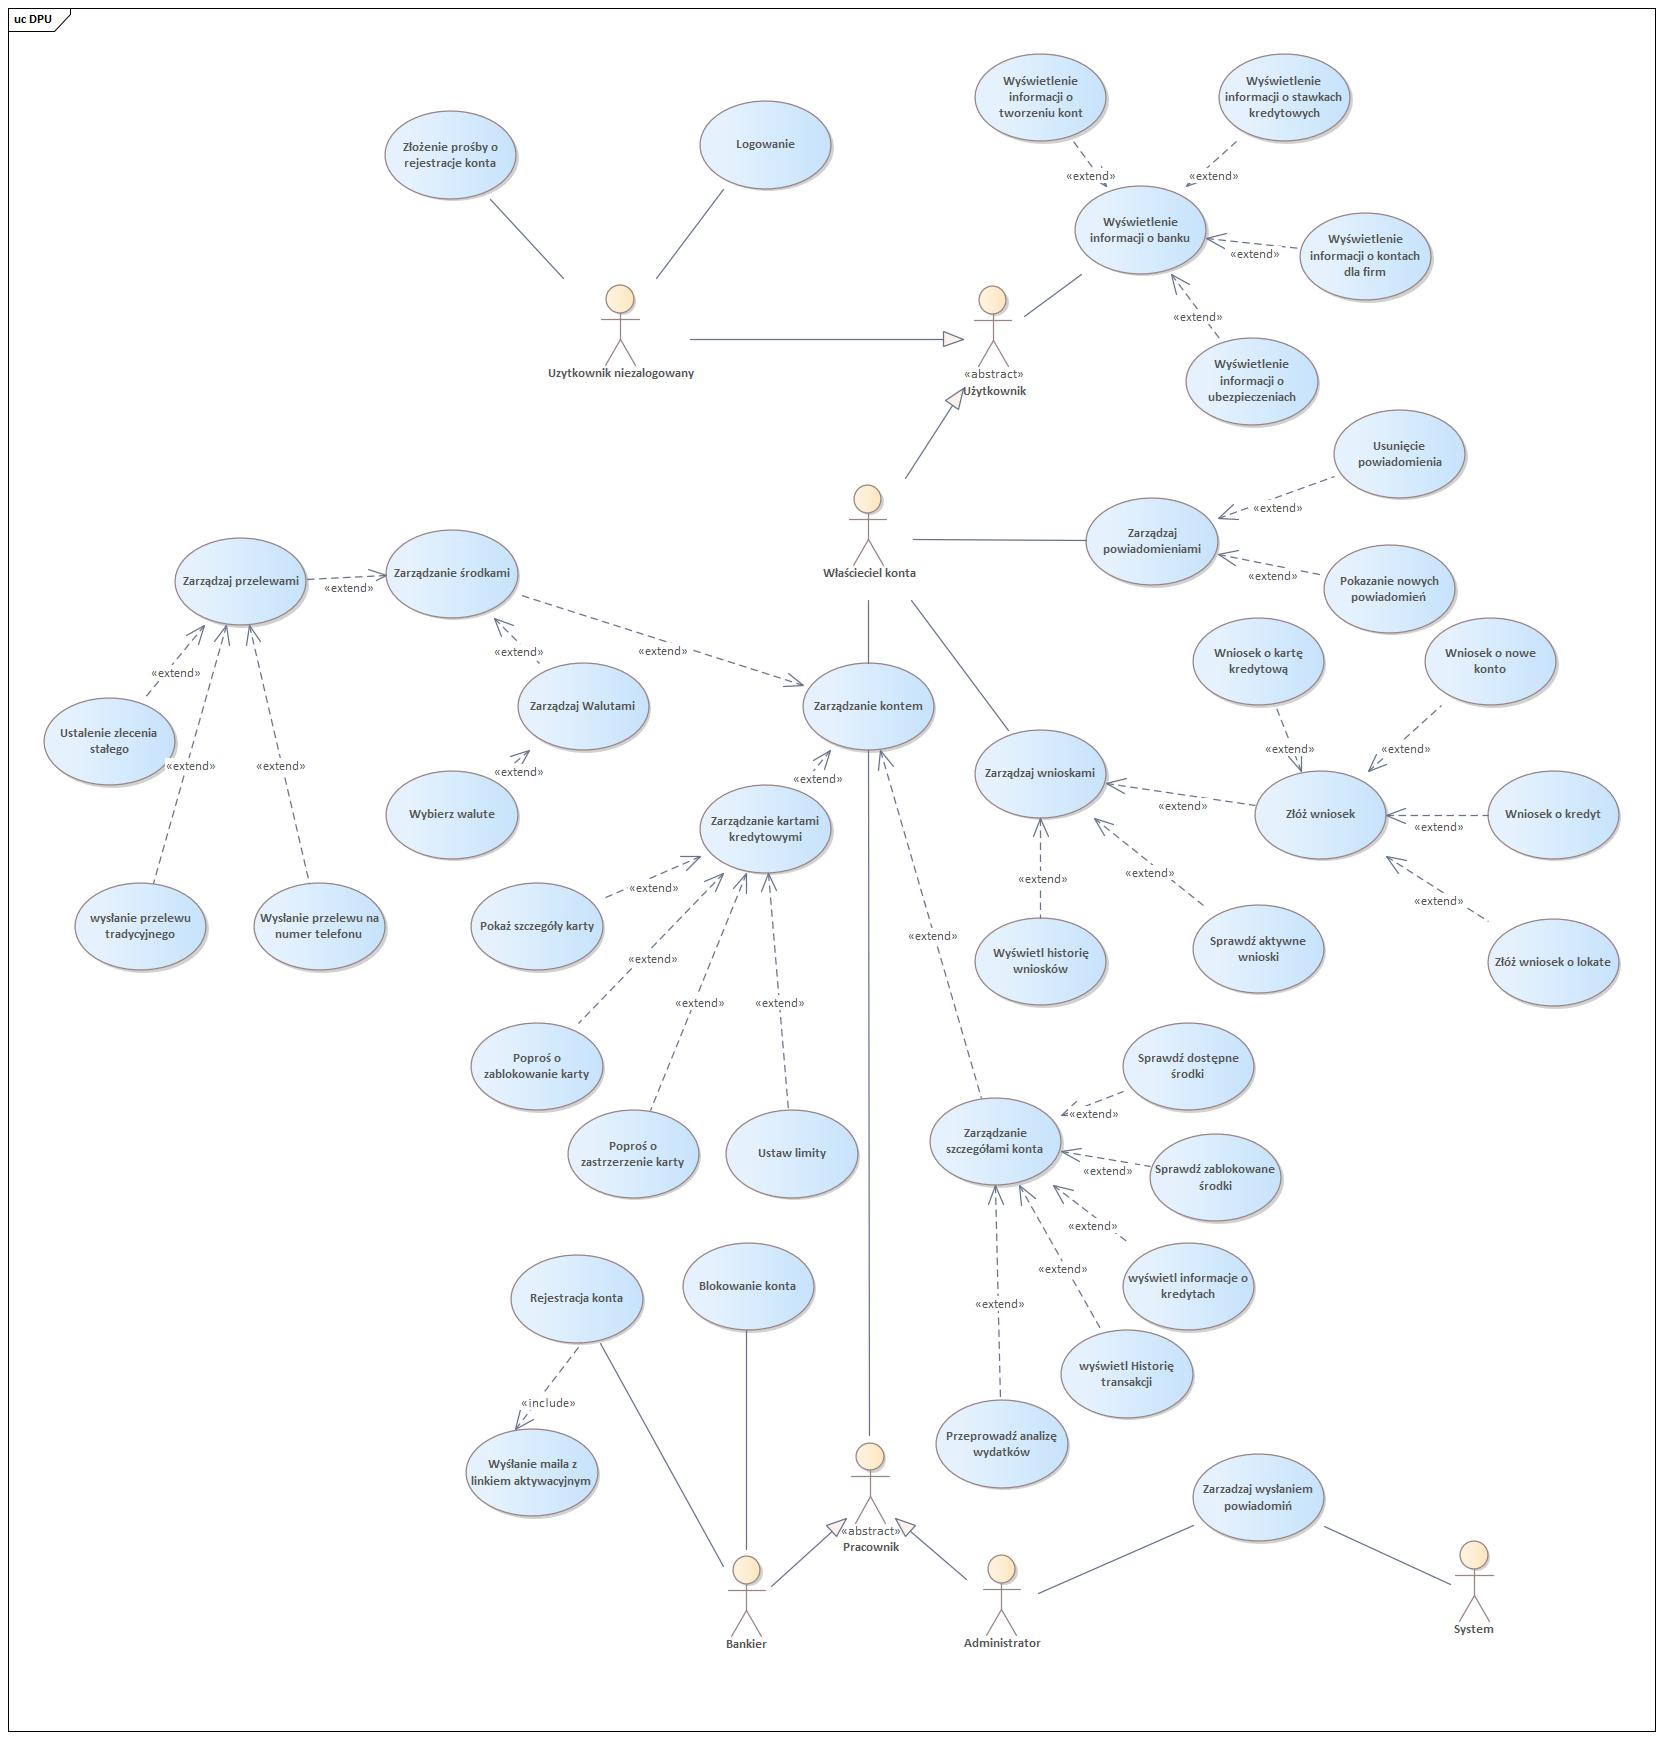
\includegraphics[width=1\textwidth]{images/DPU.jpg}
	\caption{Diagram przypadków użycia}
	\label{fig:UseCase}
\end{figure}
\section{Diagram stanów}
\begin{figure}[H]
	\centering
	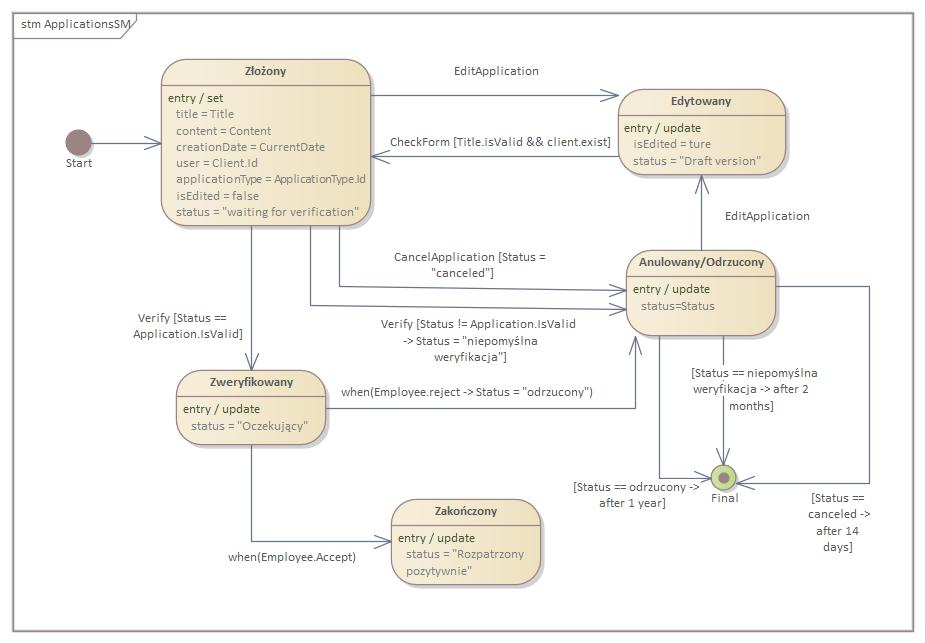
\includegraphics[width=1\textwidth]{images/Wniosek.jpg}
	\caption{Diagram stanów składania wniosku}
	\label{fig:StateMachine}
\end{figure}
\section{Diagramy sekwencji}
\begin{figure}[H]
	\centering
	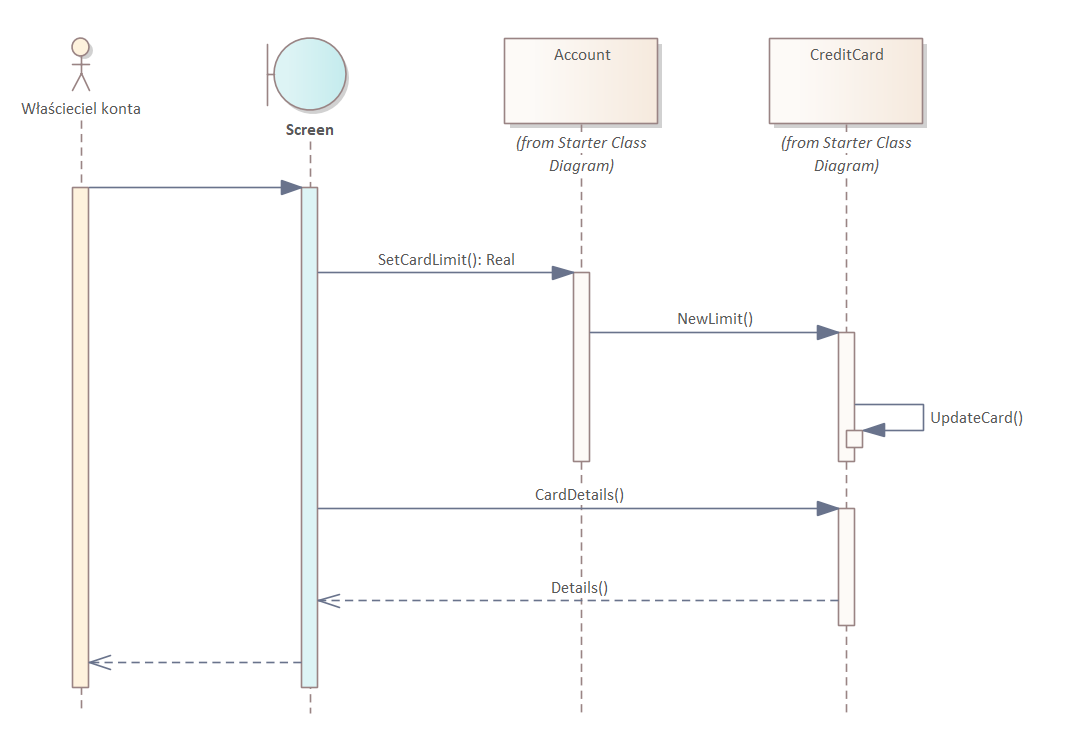
\includegraphics[width=0.7\textwidth]{images/Limit.png}
	\caption{Diagram sekwencji Limit}
	\label{fig:Seq1}
\end{figure}
\begin{figure}[H]
	\centering
	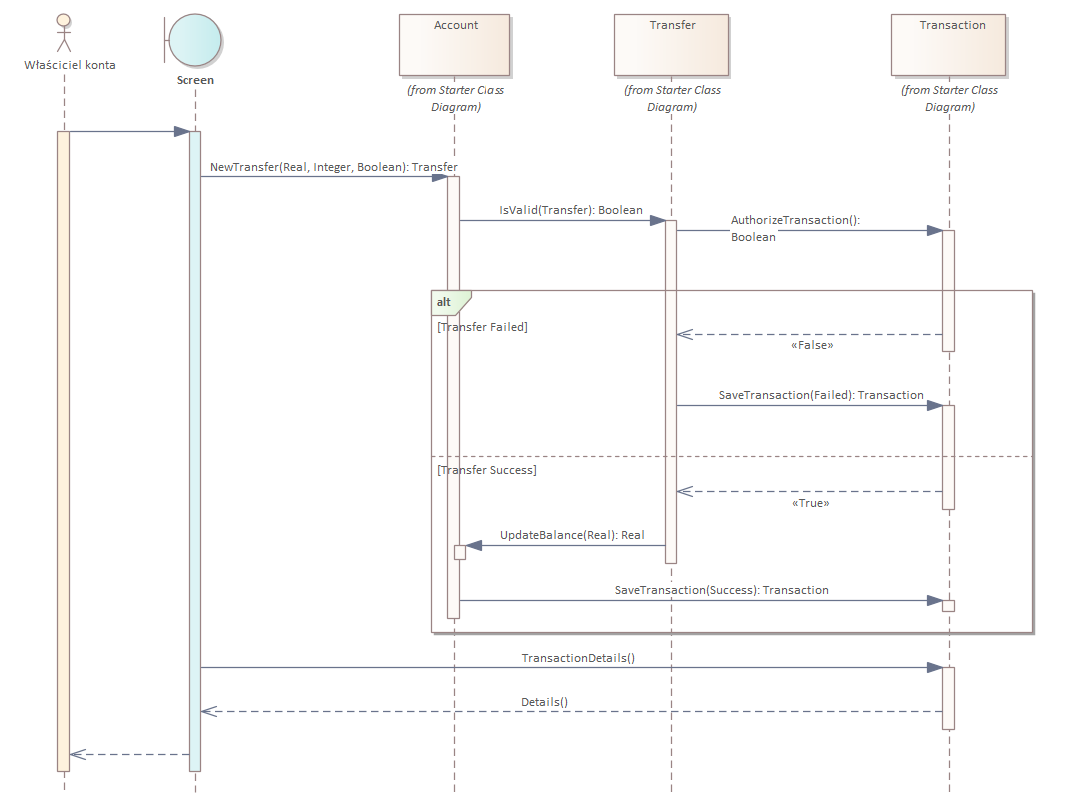
\includegraphics[width=0.7\textwidth]{images/Przelew.png}
	\caption{Diagram sekwencji Przelew}
	\label{fig:Seq2}
\end{figure}